\documentclass[12pt,a4paper]{article}
\usepackage[utf8]{inputenc}
\usepackage[margin=0.5in]{geometry}
\usepackage{amsmath}
\usepackage{amsfonts}
\usepackage{amssymb}
\usepackage{amsthm}
\usepackage{graphicx}
\renewcommand{\theenumi}{\alph{enumi}}
\usepackage{needspace}
%%\def\item{\needspace{\baselineskip}\svitem}
\begin{document}
	
	\subsection*{Question 1}
	\begin{enumerate}
		\item
			\begin{center}
				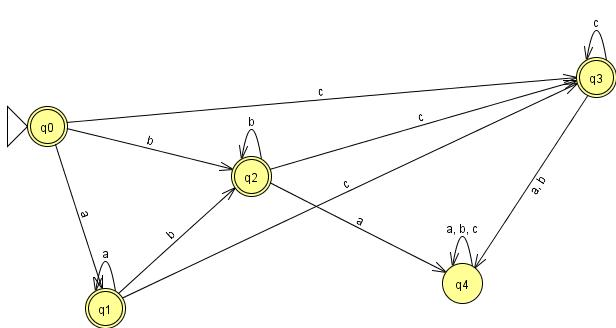
\includegraphics[width=0.7\linewidth]{../JFLAP-Automatas/a1q1a}
			\end{center}
		\item  ~\\		
			\begin{center}
				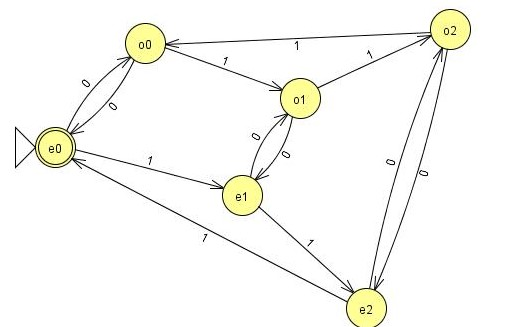
\includegraphics[width=0.7\linewidth]{../JFLAP-Automatas/a1q1b}
			\end{center}
		
		\begingroup\interlinepenalty=10000
		\item  	~\\ 
		\begin{center}
			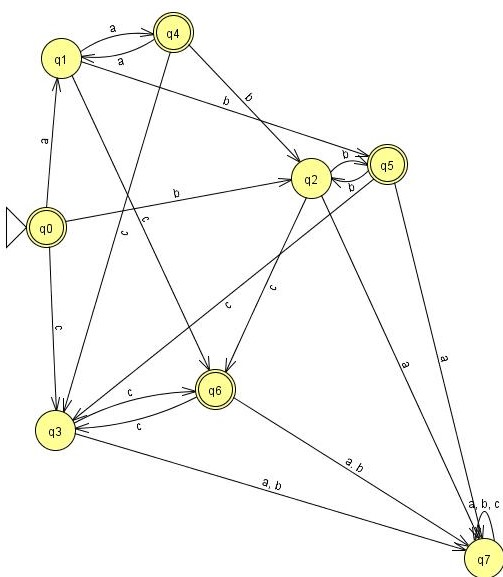
\includegraphics[width=.7\linewidth]{../JFLAP-Automatas/a1q1c}
		\end{center}
		\item  ~\\		
		\begin{center}
			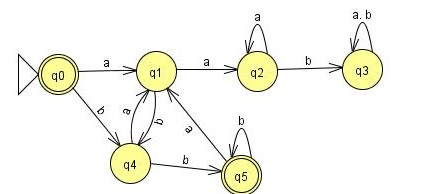
\includegraphics[width=.7\linewidth]{../JFLAP-Automatas/a1q1d}
		\end{center}
		\endgroup
	\end{enumerate}

	\subsection*{Question 2}
		\noindent
		\textbf{Base:} Let $ y=\epsilon $ then $ |y|=0$
		\begin{align*}
			&\hat{\delta}(\hat{\delta}(q,x),y)		\tag{assumption}
			\\ &=\hat{\delta}(\hat{\delta}(q,x),\epsilon)	\tag{definition}
			\\ &=\hat{\delta}(q,x)					\tag{definition}
			\\ &=\hat{\delta}(q,x\epsilon)			\tag{definition}
			\\ &=\hat{\delta}(q,xy) 				\tag{assumption}
			\\ &Q.E.D.
		\end{align*}
		
		\noindent
		\textbf{IH:} if $|y|=n$ then $\hat{\delta}(q,x)=\hat{\delta}(\hat{\delta}(q,x),y)$\\
		
		\noindent
		\textbf{IS:} Assume the hypothesis is true for $n$. We will show that it is true for $n+1$ 
		\noindent
		Let $y=|za|$ where $z$ is a string such that $|z| \ge 0$ and $a$ is a character in $\Sigma$
		\begin{align*}
			&\hat{\delta}(\hat{\delta}(q,x),y)				\tag{assumption $y=za$}
			\\ &= \hat{\delta}(\hat{\delta}(q,x),za) 		\tag{assumption}
			\\ &= \delta(\hat{\delta}(\hat{\delta}(q,x),y),a) \tag{definition $\hat{\delta}$}
			\\ &= \delta(\hat{\delta}(q,xz),a)				\tag{IH}
			\\ &= \hat{\delta}(q,xza)						\tag{definition $\hat{\delta}$}
			\\ &= \hat{\delta}(q,xy)						\tag{assumption $y=za$}
			\\ &Q.E.D
		\end{align*}
	
	\subsection*{Question 3}
		\begin{center}
			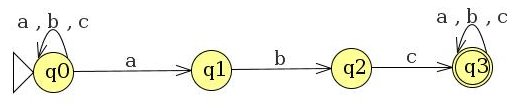
\includegraphics[width=0.7\linewidth]{a1q3}
		\end{center}

	\subsection*{Question 4}
		\begin{enumerate}
			\item ~\\
				\begin{center}
					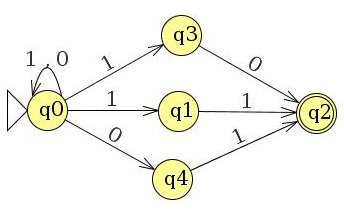
\includegraphics[width=0.5\linewidth]{a1q4nfa}
				\end{center}
			\item ~\\
			\begin{center}
				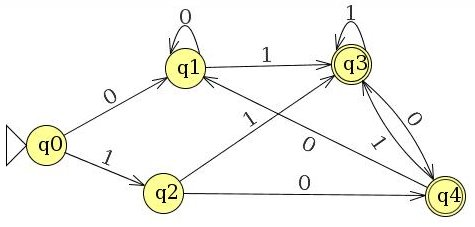
\includegraphics[width=0.7\linewidth]{a1q4dfa}
			\end{center}
		\end{enumerate}
	
	\subsection*{Question 5}	
		\begin{table}[h]
			\centering
			\begin{tabular}{|c|c|c|}
				\hline
				 & 0 & 1 \\
				\hline
				$\rightarrow$ p & \{q,s\} & $\emptyset$\\
				q & \{r\} & \{s\}\\
				r & $\emptyset$ & \{s\}\\
				*s & $\emptyset$ & $\emptyset$\\
				\hline
			\end{tabular}
		\end{table}
		
		\begin{center}
			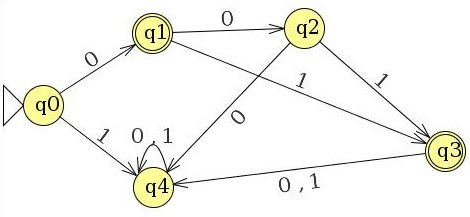
\includegraphics[width=0.7\linewidth]{a1q5}
		\end{center}

	\subsection*{Question 6}
		

\end{document}
